\chapter{Explorationsalgorithmus}
Mit diesen Voraussetzungen kann eine Komponente entwickelt werden, welche die Erwartungen der nachfragenden Komponente mit den bestehenden Funktionalit�ten der angebotenen Komponenten zusammenbringt. In \abbref{common_structure} ist dies als Explorationskomponente dargestellt. Die Abh�ngigkeiten zu der nachfragenden und den angebotenen Komponenten ist nicht direkt vorhanden, da sie lediglich durch reflexive Aufrufe zur Laufzeit zustande kommen.
\myBigFigure{common_structure}{Allgemeiner Aufbau des System mit der Explorationskomponente}{common_structure}
\noindent
Um die Explorationskomponente anzusprechen, muss der Entwickler eine Instanz der Klasse DesiredComponentFinder, die von der Explorationskomponente bereitgestellt wird, erzeugen. Dabei m�ssen dem Konstruktor dieser Klasse zwei Parameter �bergeben werden. Der erste Parameter ist eine Liste aller angebotenen Interfaces. Der zweite Parameter ist eine java.util.Function, �ber die die konkreten Implementierungen der angebotenen Interfaces ermittelt werden k�nnen. Die Suche wird mit dem Aufruf der Methode getDesiredComponent gestartet, welcher das erwartete Interface als Parameter �bergeben werden muss. Somit kann ein Objekt der Klasse DesiredComponentFinder f�r mehrere Suchen mit unterschiedlichen erwarteten Interfaces verwendet werden.\\\\
Zu erw�hnen ist noch, dass die in der nachfragenden Komponente spezifizierten Erwartungen mitunter nur durch eine Kombination von angebotenen Komponenten erf�llt werden k�nnen. Aus diesem Grund wird innerhalb der Explorationskomponente eine so genannte ben�tigte Komponente erzeugt, in der das Zusammenspiel einer solchen Kombination von angebotenen Komponenten verwaltet wird. Ein solches Szenario ist \abbref{combinated_components} zu entnehmen.
\myBigFigure{combinated_components}{Kombination von angebotenen Komponenten}{combinated_components}
\noindent
Die Suche nach einer ben�tigten Komponente innerhalb der Explorationskomponente erfolgt in zwei Schritten. Im ersten Schritt werden die angebotenen Interfaces hinsichtlich ihrer Struktur mit dem erwarteten Interface abgeglichen. Im zweiten Schritt werden die Ergebnisse aus dem ersten Schritt hinsichtlich der semantischen Tests �berpr�ft. Dieser mehrstufige Ansatz baut auf der Arbeit von Hummel \cite{hummel08} auf.
\subsection{1. Stufe - Strukturelle �bereinstimmung}
Wie in \cite{hummel08} wird in der ersten Stufe der Suche versucht die angebotenen Interfaces herauszusuchen, die strukturell mit dem erwarteten Interface �bereinstimmen. Zu diesem Zweck werden Type-Matcher verwendet, durch die festgestellt werden kann, ob sich ein Typ in einen anderen Typ konvertieren l�sst. Die Konvertierung erfolgt auf Objekt-Ebene �ber Proxies, die ihre Methodenaufrufe delegieren.\\\\\
So wird bspw. bei der Konvertierung eines Objektes von TypA (ObjA) in ein Objekt von TypB (ObjB) ein Proxy-Objekt f�r TypB erzeugt (ProxyB), welcher die Methodenaufrufe an ObjA delegiert (vgl. auch \abbref{combinated_components}).\\\\
Hummel hatte hierzu bereits auf einige Matcher von Moormann Zaremski \cite{moormann} zur�ckgegriffen, die in dieser Arbeit ebenfalls zum Einsatz kommen. Die Definitionen der Matcher beziehen sich auf die Programmiersprache Java, wodurch grundlegend von einer nominalen Typkonformit�t ausgegangen wird.
\subsubsection{Notation zur Beschreibung der Matcher}
Die �bereinstimmung bzw. das Matching zweier Typen $ A $ und $ B $ �ber einen Matcher $ M $ wird in dieser Arbeit mit $\matchTyp{A}{M}{B}$ notiert. Weiterhin wird die Identit�t zweier Typen mit $ A = B $ beschrieben. Eine Vererbungshierarchie, in der $ A $ von $ B $ erbt, wird mit $\inhTyp{A}{B}$ beschrieben. Au�erdem ist die Adressierung der Typen von Attributen, die innerhalb eines Typs verwendet werden, notwendig. F�r die Adressierung des Typs eines Attributs $ a $ im Typ $ A $ wird $\selTyp{A}{a}$ geschrieben. Die logische Verkn�pfung der einzelnen Elemente der Sprache �ber die Quantoren und Junktoren der Pr�dikatenlogik 1. Stufe ist ebenfalls m�glich.\\\\
Die Konvertierung eines Typs $ A $ in einen Typ $ B $ wird, wie bereits erw�hnt, auf technischer Ebene �ber Proxies umgesetzt. Von daher kann die Beschreibung des Konvertierungsverfahrens eines Matchers auf die Beschreibung der Delegation einzelner Methoden beschr�nkt werden. Hierf�r wird folgende Notation verwendet:\\\\
Eine Methode $m$ enth�lt einen R�ckgabetyp $ RT $ und eine Menge von Parametertypen $ PT $. Die Menge der Parametertypen wird zur besseren Lesbarkeit auf einen Parametertyp beschr�nkt. Der Aufruf einer Methode $ m $ eines Typs $ A $ mit dem R�ckgabetyp $ RT $ und dem Parametertyp $ PT $ wird mit $ A.m( PT ) : RT $ notiert. Sofern die Konvertierung keinen Einfluss auf den R�ckgabetyp oder die Parametertypen hat, wird dies verk�rzt mit $ A.m $ beschrieben.\\\\
Die Delegation von Methodenaufrufen eines Typs wird mit dem Operator $\Rightarrow$ beschrieben. F�r eine Delegation des Aufrufs einer Methode $ m $ des Typs $ A $, welcher an einen Typ $ B $ und dessen Methode $ n $ delegiert wird, schreibt man $\delegate{A.m}{B.n}$. Ferner ist hierbei zwischen einem Source- und einem Target-Typ zu unterscheiden. Der Source-Typ befindet sich links vom Operator ($\Rightarrow$). Auf diesem Typ findet der Methodenaufruf statt. Der Target-Typ befindet sich auf der rechten Seite des Operators ($\Rightarrow$). Dieser stellt das Ziel der Delegation dar. Da bei der Delegation mitunter weitere (interne) Matcher zur Anwendung kommen m�ssen, wird hierf�r ebenfalls eine Notation ben�tigt. Daher soll die Konvertierung eines Typs $ A $ in einen Typ $B$ wird mit $\applyMatcher{B}{A}$ beschrieben. Als Voraussetzung f�r diese Konvertierung muss $\matchTyp{A}{M}{B}$ gelten.\\\\
Die folgenden Matcher werden jeweils durch ein Szenario motiviert. In den dazugeh�rigen Diagrammen ist das Object des Source-Typs (Source-Objekt) jeweils mit \emph{source} und das Objekt des Target-Typs (Target-Objekt) jeweils mit \emph{target} bezeichnet. Um die Verwendung der Implementierungen der einzelnen Matcher in Verbindung mit diesem Szenario nachvollziehen zu k�nnen, wird jeweils auf einen Abschnitt aus Anhang \ref{matcherExamples} verweisen. Dort sind Code-Beispiele f�r die Verwendung der Matcher in Bezug auf das jeweilige Szenario mit entsprechenden Nachbedingungen hinterlegt.\\\\
Die Definitionen der Matcher bestehen jeweils aus zwei Teilen. Der erste Teil (�bereinstimmung) definiert, unter welchen Bedingungen �ber den entsprechenden Matcher zwei Typen als �bereinstimmend gelten. Der zweite Teil (Konvertierung) beschreibt, wie die Delegation der Aufrufe von Methoden, die vom Source-Typ spezifiziert werden, an die Methoden, die vom Target-Typ spezifiziert werden.

\subsubsection{ExactTypeMatcher}\label{exactTypeMatcher}
\myparagraph{Szenario}
Dieser Matcher stellt das Matching zweier identischer Typen fest. In dem Szenario wird von zwei Objekten vom Typ SuperClass ausgegangen. Die Klasse SuperClass ist in \abbref{cd_superclass} dargestellt. Der Aufruf einer Methode auf dem Source-Objekt f�hrt zu einer Delgation der Methode an das Target-Objekt (siehe \abbref{sd_exact_super}).
\begin{figure}[H]
\begin{minipage}[b]{.33\linewidth}
  \centering
  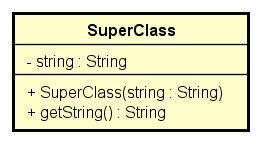
\includegraphics[width=\linewidth]{cd_superclass}
  \caption{SuperClass}
  \label{abb:cd_superclass}

\end{minipage}%
\hspace{.04\linewidth}% Abstand zwischen Bilder
\begin{minipage}[b]{.63\linewidth}


  \centering
  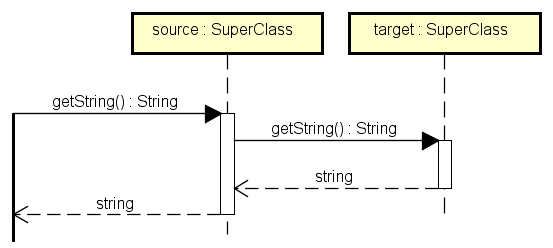
\includegraphics[width=\linewidth]{sd_exact_super}
  \caption{Szenario ExactTypeMatcher}
  \label{abb:sd_exact_super}

\end{minipage}
\end{figure}

\myparagraph{Definition}
\begin{matcherEquivDef}{ExactTypeMatcher}
\matchTyp{A}{exact}{B} \text{ wenn } A = B
\end{matcherEquivDef}
\begin{matcherConvDef}{ExactTypeMatcher}{
Sei $ m $ eine Methode des Typen $ A $ und $ B $.}
\delegate{A.m}{B.m}
\end{matcherConvDef}\\
Ein Beispiel f�r die Verwendung des Matchers ist in \appref{exactMatcherExample} zu finden.
\subsubsection{GenTypeMatcher}\label{genTypeMatcher}
\myparagraph{Szenario}
Dieser Matcher stellt das Matching zwischen zwei Typen her, die in einer Vererbungsbeziehung stehen. Speziell erlaubt dieser Matcher das Matching eines Supertyps als Source-Typen mit einem Subtypen als Target-Typen. In dem Szenario wird neben dem Typ SuperClass aus \abbref{cd_superclass} von einem weiteren Typen SubClass ausgegangen. Dabei stehen diese beiden Typen in einer Vererbungsbeziehnung, die in \abbref{cd_subclass_extends_superclass} dargestellt wird. Der Aufruf einer Methode auf dem Source-Objekt f�hrt zu einer Delgation der Methode an das Target-Objekt (siehe \abbref{sd_gen_super2sub}).
\begin{figure}[H]
\begin{minipage}[b]{.33\linewidth}
  \centering
  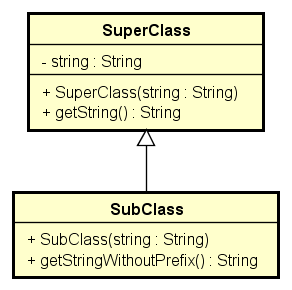
\includegraphics[width=\linewidth]{cd_subclass_extends_superclass}
  \caption{Beziehung zwischen SuperClass und SubClass}
  \label{abb:cd_subclass_extends_superclass}

\end{minipage}%
\hspace{.04\linewidth}% Abstand zwischen Bilder
\begin{minipage}[b]{.63\linewidth}


  \centering
  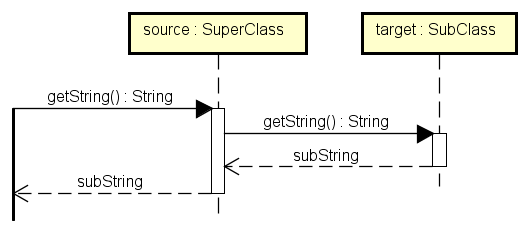
\includegraphics[width=\linewidth]{sd_gen_super2sub}
  \caption{Szenario GenTypeMatcher}
  \label{abb:sd_gen_super2sub}

\end{minipage}
\end{figure}




\myparagraph{Definition}
\begin{matcherEquivDef}{GenTypeMatcher}
\matchTyp{A}{gen}{B} \text{ wenn } \inhTyp{B}{A}
\end{matcherEquivDef}
\begin{matcherConvDef}{GenTypeMatcher}{
Sei $ m $ eine Methode des Typs $ A $, die aufgrund der Vererbung auch von Typ $ B $ bereitgestellt wird.}
\delegate{A.m}{B.m}
\end{matcherConvDef}\\
Ein Beispiel f�r die Verwendung des Matchers ist in \appref{genMatcherExample} zu finden.

\subsubsection{SpecTypeMatcher}\label{specTypeMatcher}
\myparagraph{Szenario}
Analog zum GenTypeMatcher stellt der SpecTypeMatcher ebenfalls das Matching zwischen Typen fest, die in einer Vererbungsbeziehung stehen. Allerdings ist der Source-Typ in diesem Matcher der Subtyp und der Target-Typ der Supertyp. In dem Szenario wird wiederum von den Klassen SuperClass und SubClass aus \abbref{cd_subclass_extends_superclass} ausgegangen. Der Methodenaufruf erfolgt hier aber auf dem Subtypen und wird an den Supertypen delegiert (siehe \abbref{sd_spec_sub2super}).
\myScalableFigure[0.7\linewidth]{sd_spec_sub2super}{Szenario SpecTypeMatcher}{sd_spec_sub2super}
\noindent
Dabei sind zwei Methodenaufrufe auf dem Subtyp beschrieben. W�hrend der Aufruf der Methode getString erfolgreich delegiert werden kann, f�hrt der Aufruf der Methode getStringWithoutPrefix zu einem Laufzeitfehler, da der Matcher keine passende Methode in dem Target-Typ ermitteln kann. Dieses Problem tritt bei allen Methoden auf, die nicht vom Supertyp an den Subtyp vererbt oder �berschrieben wurden.\footnote{Anders gesagt, erm�glicht dieser Matcher einen Downcast, bei dem ein Objekt eines allgemeinen Typen auf einen spezielleren Typen gecastet wird. Das Problem bzgl. des fehlschlagenden Methodenaufrufs in der beschriebene Form ist bei einem Downcast allgegenw�rtig.} Aus diesem Grund muss diese Bedingung in der Definition der Konvertierung dieses Matchers mit aufgenommen werden.
\myparagraph{Definition}
\begin{matcherEquivDef}{SpecTypeMatcher}
\matchTyp{A}{genspec}{B} \text{ wenn } \inhTyp{A}{B}
\end{matcherEquivDef}
\begin{matcherConvDef}{SpecTypeMatcher}{
Sei $ m $ eine Methode des Typs $ A $, die von $ B $ an $ A $ vererbt wurde.}
\delegate{A.m}{B.m}
\end{matcherConvDef}\\
Ein Beispiel f�r die Verwendung des Matchers ist in \appref{specMatcherExample} zu finden.
\subsubsection{WrappedTypeMatcher}\label{wrappedTypeMatcher}
\myparagraph{Szenario}
Die bisherigen Type-Matcher sind in der Lage das Matching f�r zwei Typen festzustellen, ohne daf�r R�cksicht auf deren innere Struktur nehmen zu m�ssen. Dies ist f�r identische oder hierarchisch organisierte Typen auch nicht notwendig. Es ist jedoch auch denkbar, dass sich beiden Typen auf anderem Wegen assoziieren lassen. Ein Beispiel daf�r w�re Boxed- bzw. - noch allgemeiner gefasst - Wrapper-Typen. In \abbref{cd_subclass_subwrapper} sind zwei Klassen dargestellt, die in einer solchen Beziehung zueinander stehen. Bez�glich des Matchings sind auch hier wiederum zwei F�lle zu unterscheiden. Der erste Fall, in dem das Matching des Source-Typen SubClass mit dem Typen eines Attributs wrapped des Traget-Typen SubWrapper festgestellt werden kann, ist in \abbref{sd_wrapped_sub2subwrapped} dargestellt.
\begin{figure}[H]
\begin{minipage}[b]{.33\linewidth}
  \centering
  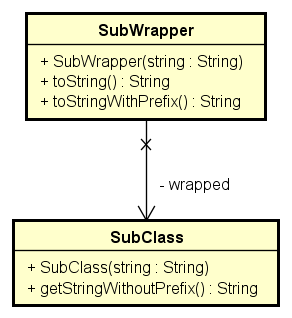
\includegraphics[width=\linewidth]{cd_subclass_subwrapper}
  \caption{Beziehung zwischen SubClass und SubWrapper}
  \label{abb:cd_subclass_subwrapper}

\end{minipage}%
\hspace{.04\linewidth}% Abstand zwischen Bilder
\begin{minipage}[b]{.63\linewidth}


  \centering
  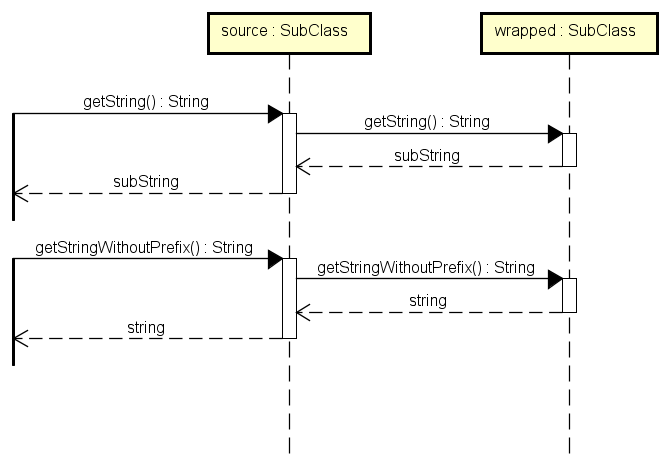
\includegraphics[width=\linewidth]{sd_wrapped_sub2subwrapped}
  \caption{Szenario WrappedTypeMatcher}
  \label{abb:sd_wrapped_sub2subwrapped}

\end{minipage}
\end{figure}
\noindent
Der WrappedTypeMatcher stellt das Matching f�r ein solches Szenario fest. Das Matching der beiden Typen beruht letztendlich auf einem Matching zwischen dem Source-Type und dem Typen eines Attributs des Target-Typs. Der Matcher, �ber den dieses Matching innerhalb des WrappedTypeMatchers festgestellt wird, wird als interner Matcher bezeichnet. In dem Szenario aus \abbref{sd_wrapped_sub2subwrapped} wird als interner Matcher der bereits beschriebene ExactTypeMatcher verwendet, weil der Source-Type und der Typ des Attributs wrapped identisch sind.
\myparagraph{Definition}
\begin{matcherEquivDef}{WrappedTypeMatcher}
\matchTyp{A}{wrapped}{B} \text{ wenn } \exists \selTyp{B}{attr} : \matchTyp{A}{M}{attr}
\end{matcherEquivDef}\\
Der zuvor genannte interne Matcher wird in der Definition mit $M$ beschrieben, was stellvertretend f�r eine Menge von Matchern steht. Als interne Matcher kommen hierbei der ExactTypeMatcher, der GenTypeMatcher und der SpecTypeMatcher in Frage.\\
\begin{matcherConvDef}{WrappedTypeMatcher}{
Sei $m$ eine Methode des Typs $A$. Sei weiterhin $B$ ein Typ, der ein Attribut vom Typ $attr$ enth�lt, f�r den gilt $\matchTyp{A}{M}{attr}$.
}
\delegate{A.m}{(\applyMatcher{A}{attr}).m}
\end{matcherConvDef}\\
Ein Beispiel f�r die Verwendung des Matchers in Bezug auf das o.g. Szenario ist in \appref{wrappedMatcherExample} zu finden. Au�erdem sind dort auch weitere Szenarien aufgef�ht, in denen der GenTypeMatcher oder der SpecTypeMatcher als interner Matcher zur Anwendung kommen.


\subsubsection{WrapperTypeMatcher}\label{wrapperTypeMatcher}
\myparagraph{Szenario}
Dieser Matcher stellt das Pendant zum WrappedTypeMatcher dar. Der Unterschied bzgl. des Szenarios besteht darin, dass nun der Source-Typ derjenige ist, der ein Attribut enth�lt, f�r dessen Typ ein Matching zum Target-Typen �ber den ExactTypeMatcher, den GenTypeMatcher oder den SpecTypeMatcher festgestellt werden kann. F�r das Szenario ist wiederum von den Typen aus \abbref{cd_subclass_subwrapper} auszugehen. Die Delegation der m�glichen Methodenaufrufe am Source-Typen, sind in \abbref{sd_wrapper_subwrapped2sub} abgebildet. Hierbei ist hervorzuheben, dass zur Laufzeit das Objekt vom Target-Typen in das Attribut des Objektes vom Source-Typen injiziert wird. Dies soll in \abbref{sd_wrapper_subwrapped2sub} durch die Bezeichnung des Targets mit wrapped (dem Namen des Attributs) und target dargestellt werden. Eine Methoden-Delegation findet nur dann statt, wenn sie auch im Wrapper-Typen (Source-Typen) implementiert wurde\footnote{Implementierung von SubWrapper: siehe \appref{matcherExamples} \lstref{LST_subwrapper_impl}}.
\myScalableFigure[0.8\linewidth]{sd_wrapper_subwrapped2sub}{Szenario WrapperTypeMatcher}{sd_wrapper_subwrapped2sub}
\myparagraph{Definition}
\begin{matcherEquivDef}{WrapperTypeMatcher}
\matchTyp{A}{wrapper}{B} \text{ wenn } \exists\selTyp{A}{attr} : \matchTyp{B}{M}{attr} 
\end{matcherEquivDef}\\
Wie an dieser Beschreibung zu erkennen ist, werden auch hier wieder ein interner Matcher $M$ verwendet. Analog zum WrappedTypeMatcher kommen auch hier der ExactTypeMatcher, der GenTypeMatcher und der SpecTypeMatcher in Frage.\\
\begin{matcherConvDef}{WrappedTypeMatcher}{
Sei $m$ eine Methode des Typs $A$.
}
\delegate{A.m}{A.m}
\end{matcherConvDef}\\
Ein Beispiel f�r die Verwendung des Matchers in Bezug auf das o.g. Szenario ist in \appref{wrapperMatcherExample} zu finden. Au�erdem sind dort auch weitere Szenarien aufgef�ht, in denen der GenTypeMatcher oder der SpecTypeMatcher als interner Matcher zur Anwendung kommen.

\subsubsection{StructuralTypeMatcher}\label{structTypeMatcher}
Die bisher beschriebene Type-Matcher erlauben lediglich ein Matching zwischen Typen, die syntaktisch miteinander in einer direkten Beziehung stehen. Ein Ziel dieser Arbeit ist es jedoch Typen, die voneinander syntaktisch unabh�ngig sind, miteinander zu matchen, um darauf aufbauend, deren Semantik zu �berpr�fen. Hierf�r soll wie auch in \cite{hummel08} die strukturelle �bereinstimmung der beiden Typen ermittelt und verwendet werden. Diesem Zweck dient der StructuralTypeMatcher.
\myparagraph{Szenario}
Um die grundlegenden Eigenschaften des StructuralTypeMatchers darzustellen, wird von einem Szenario ausgegangen, in dem der Target-Typ (angebotenes Interface) zu jeder Methode des Sources-Typs (ben�tigtes Interface) eine passende Methode anbietet. Eine Kombination von angebotenen Interfaces ist somit in diesem Szenario nicht notwendig.\\\\
\abbref{cd_superrsubp_subrsuperp} zeigt die Typen, von denen in dem folgenden Szenario ausgegangen wird. Hierbei sind zwei Klassen aufgef�hrt, die jeweils zwei Methoden anbieten. Die Parameter- und R�ckgabetypen der Methoden sind aus den Szenarien zu den anderen Matchern bekannt. Die Klasse SuperReturnSubParamClass wird in dem folgenden Szenario als Source-Typ und die Klasse SubReturnSuperWrapperParamClass wird als Target-Typ verwendet. Um die strukturelle �bereinstimmung der beiden Typen festzustellen, muss der StructuralTypeMatcher ein Matching zwischen den Parameter- und R�ckgabetypen der einzelnen Methoden herstellen. Dies erfolgt wiederum �ber interne Type-Matcher. An dieser Stelle k�nnen alle zuvor genannten Type-Matcher als interner Type-Matcher verwendet werden. Die Delegation der Methode-Aufrufe erfolgt dann an die Methode des Target-Objekts, die als �bereinstimmende bzw. passende Methode ermittelt wurde (siehe \abbref{sd_struct}). Da beide Methoden eine unterschiedliche Anzahl von Parametern haben, ist in diesem Beispiel leicht nachzuvollziehen, welche Methoden zusammenpassen. Als interner Type-Matcher wurde in diesem Szenario der GenTypeMatcher verwendet. 
\myBigFigure{cd_superrsubp_subrsuperp}{SuperReturnSubParamClass und SubReturnSuperParamClass}{cd_superrsubp_subrsuperp}
\myBigFigure{sd_struct}{Szenario StructTypeMatcher}{sd_struct}
\myparagraph{Definition}
\begin{matcherEquivDef}{StructuralTypeMatcher}
&\matchTyp{A}{struct}{B} \text{ wenn}\\
&\exists(A.m(MP) : MR) : \exists (B.n(NP):NR):\matchTyp{MP}{P}{NP} \wedge \matchTyp{NR}{R}{MR}
\end{matcherEquivDef}\\
Da die Notation es nicht hergibt, ist zus�tzlich zu erw�hnen, dass die Reihenfolge der Parameter in $m$ und $n$ irrelevant ist.\\
%fuer Formatierung
\\
\begin{matcherConvDef}{StructuralTypeMatcher}{
Sei $m$ eine Methode des Typs $A$.\\
Der R�ckgabetyp von $m$ sei $MR$ und $MP$ der Parametertyp von $m$.\\
Weiterhin sei $n$ eine Methode des Typs $B$.\\
Der R�ckgabetyp von $n$ sei $NR$ und $NP$ der Parametertyp von $n$.
}
\delegate{A.m(MP):MR}{B.n(\applyMatcher{NP}{MP}) : \applyMatcher{MR}{NR}}
\end{matcherConvDef}\\
Ein Beispiel f�r die Verwendung des Matchers in Bezug auf das o.g. Szenario ist in \appref{structMatcherExample} zu finden. Au�erdem sind dort auch weitere Szenarien aufgef�ht, in denen andere Matcher als interner Matcher zur Anwendung kommen.

\subsubsection{Typ- und Methoden-Konvertierungsvarianten}\label{type_meth_conv}
Die Konvertierung der einzelnen Type-Matcher liefert eine Menge von so genannten Typ-Konvertierungsvarianten. Eine Typ-Konvertierungsvariante beschreibt eine M�glichkeit, wie ein Typ in einen anderen konvertiert werden kann. Zu diesem Zweck enth�lt eine Typ-Konvertierungsvariante zwei Arten von Information: 
\begin{enumerate}
\item Objekterzeugungsrelevante Informationen
\item Methodendelegationsrelevante Informationen
\end{enumerate}
Typ-Konvertierungsvarianten werden von einem konkreten Typ-Matcher f�r jede m�gliche Form der �bereinstimmung erzeugt. Ein Matcher erzeugt, wenn �berhaupt, immer nur eine Typ-Konvertierungsvariante.\\\\
Die objekterzeugungsrelevanten Informationen sorgen daf�r, dass das Proxy-Objekt f�r den Source-Typ korrekt erzeugt werden kann.\\\\
Die methodendelegationsrelevanten Informationen werden verwendet um so genannten Methoden-Konvertierungsvarianten zu erzeugen. Diese sorgen daf�r, dass das R�ckgabe-Objekt und die Parameter-Objekte beim Methodenaufruf korrekt konvertiert werden und dass der Aufruf an die richtige Methode des Target-Typs delegiert wird.\\\\
Speziell der StructuralTypeMatcher erm�glicht es, zu einer Methode des Source-Typen mehrere methodendelegationsrelevanten Informationen zu erhalten. Das liegt daran, dass dieser Matcher alle Methoden des Source- und des Target-Typen miteinander auf �berstimmung �berpr�ft. Dabei kann es vorkommen, dass eine Methode des Source-Typen mit mehreren Methoden des Target-Typen - oder umgekehrt - �bereinstimmt.
In \abbref{konvar_voll} ist dieser Zusammenhang f�r ein angebotenes Interface AIv und einem erwarteten Interface EI, welche jeweils zwei Methoden enthalten (AM * bzw. EM *), skizziert. Hier wird angenommen, dass jede der angebotenen Methoden strukturell mit jeder der erwarteten Methoden �bereinstimmen w�rde. Dementsprechend enth�lt die Typ-Konvertierungsvariante (TKV) methodendelegationsrelevante Informationen, aus denen insgesamt 4 Methoden-Konvertierungsvarianten erzeugt werden, wovon jede eine Konvertierung entlang der eingezeichneten Pfeile erm�glicht.\\\\
Dabei gilt jedoch, aufgrund der �berlegungen zur Kombination von angebotenen Komponenten (siehe auch \abbref{combinated_components}), dass eine Typ-Konvertierungsvariante nicht zu jeder der erwarteten Methoden solche methodendelegationsrelevanten Informationen enth�lt. \abbref{konvar_unv} zeigt einen solchen Fall mit dem angebotenen Interface AIu.
\begin{figure}[H]
\begin{minipage}[b]{.48\linewidth}
  \centering
  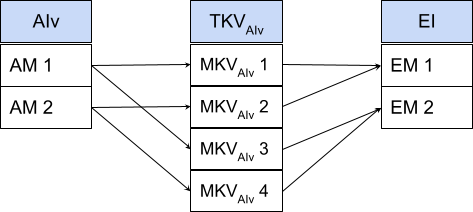
\includegraphics[width=\linewidth]{konvar_voll}
  \caption{Typ- und Methoden-Konvertierungsvarianten von AIv}
  \label{abb:konvar_voll}

\end{minipage}%
\hspace{.04\linewidth}% Abstand zwischen Bilder
\begin{minipage}[b]{.48\linewidth}


  \centering
  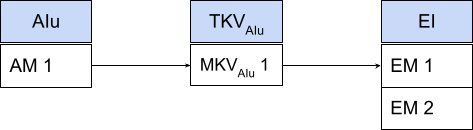
\includegraphics[width=\linewidth]{konvar_unv}
  \caption{Typ- und Methoden-Konvertierungsvarianten von AIu}
  \label{abb:konvar_unv}

\end{minipage}
\end{figure}


\section{2. Stufe - Semantische Evaluation}\label{sem_eval}
Sofern alle Typ-Konvertierungsvarianten des erwarteten Interfaces bzgl. einer Menge von angebotenen Interfaces in der 1. Stufe ermittelt wurden, k�nnen die ben�tigten Komponenten erzeugt und getestet werden.\\\\
Diese Pr�fung wird �ber die vorab spezifizierten Testf�lle des erwarteten Interfaces vorgenommen. In einem vorherigen Abschnitt wurde schon kurz beschrieben, wie eine solche Testklasse aufgebaut ist. In diesem Abschnitt wird beschrieben, wie die zu testenden ben�tigten Komponenten ermittelt werden und wie die Tests durchgef�hrt werden. 
Dies erfolgt in 6 Schritten, die im Folgenden erl�utert werden. Eine schmatische Darstellung der Semantischen Evaluation ist \abbref{flowchart_sem_eval} zu entnehmen.
\myBigFigure{flowchart_sem_eval}{Schema der semantischen Evaluation}{flowchart_sem_eval}

\subsubsection{Ermittlung der Testklassen zum erwarteten Interface}\label{sem_eval_step1}
Die Ermittlung der Testklassen erfolgt �ber die Annotation @QueryTypeTestReference, welche im erwarteten Interface spezifiziert wird. Von diesen Testklassen wird ein Testobjekt �ber den Default-Konstruktor erzeugt.
\subsubsection{Schritt 2: Kombination von Typ-Konvertierungsvarianten}\label{sem_eval_step2}
In diesem Schritt werden die ermittelten Typ-Konvertierungsvarianten miteinander kombiniert, was einer Kombination der angebotenen Interfaces gleicht. Die Anzahl $k$ der zu kombinierenden Typ-Konvertierungsvarianten kann jedoch variieren. Wenn $|EM|$ die Anzahl der Methoden im erwarteten Interface ist, gilt f�r $k$:
\begin{align*}
1 \leq k \leq |EM|
\end{align*}
\noindent
Da $k$ variabel ist, wird dieser Schritt zusammen mit allen folgenden Schritten mitunter mehrfach durchlaufen. Die Nummer des jeweiligen Iterationsschrittes wird mit $k$ gleichgesetzt. Somit wird die Anzahl der zu kombinierenden Typ-Konvertierungsvarianten mit jedem Durchlauf erh�ht. \abbref{tkv_alv_alu_1} zeigt die Kombinationen von Typ-Konvertierungsvarianten, die sich - bezogen auf die Beispiele aus \abbref{konvar_voll} und \abbref{konvar_unv} - im ersten Durchlauf ergeben. Im zweiten Durchlauf w�rde sich nur eine Kombination von Typ-Konvertierungsvarianten ergeben, da die beiden Typ-Konvertierungsvarianten von AIv und AIu miteinander kombiniert werden (siehe \abbref{comb_tkv_alv_alu_1}).



\begin{figure}[H]
\begin{minipage}[b]{.48\linewidth}
  \centering
  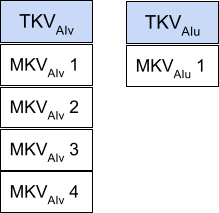
\includegraphics[width=.6\linewidth]{tkv_alv_alu_1}
  \caption{Kombinationen von Typ-Konvertierungsvarianten von AIu und AIv im ersten Durchlauf}
  \label{abb:tkv_alv_alu_1}

\end{minipage}%
\hspace{.04\linewidth}% Abstand zwischen Bilder
\begin{minipage}[b]{.48\linewidth}


  \centering
  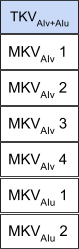
\includegraphics[width=.2\linewidth]{comb_tkv_alv_alu_1}
  \caption{Kombinationen von Typ-Konvertierungsvarianten von AIu und AIv im zweiten Durchlauf}
  \label{abb:comb_tkv_alv_alu_1}

\end{minipage}
\end{figure}

\noindent
So berechnet sich die Anzahl an ermittelten Kombinationen von Typ-Konvertierungsvarianten  ($|KombTKV|$) f�r jeden Durchlauf $k$ in Abh�ngigkeit von der Anzahl der in der 1. Stufe ermittelten Typ-Konvertierungsvarianten ($|TKV|$) wie folgt:
\begin{align*}
|KombTKV| = \frac{|TKV|! }{ (|TKV| - k)! * k!}
\end{align*}


\subsubsection{Schritt 3: Erzeugen einer ben�tigten Komponente}\label{sem_eval_step3}
Eine ben�tigte Komponente besteht aus einer Kombination von Methoden-Konvertierungsvarianten, wobei f�r jede erwartete Methode genau eine Methoden-Konvertierungsvariante innerhalb der ben�tigten Komponente existiert.\\\\
F�r die Ermittlung der Kombinationen von Methoden-Konvertierungsvarianten wird eine Kombination von Typ-Konvertierungsvarianten aus der Ergebnismenge des zweiten Schrittes im aktuellen Durchlauf  selektiert. Die daraus erzeugten Methoden-Konvertierungsvarianten werden hinsichtlich der Methoden aus dem erwarteten Interface miteinander kombiniert.\\\\
F�r die erste Kombination von Typ-Konvertierungsvarianten, die \abbref{tkv_alv_alu_1} zu entnehmen ist ($TKV_{AIv}$),  k�nnen folgende Kombinationen von Methoden-Konvertierungsvarianten erzeugt werden (siehe \abbref{comb_mkv_alv_1}).
\myBigFigure{comb_mkv_alv_1}{Kombinationen von Methoden-Konvertierungsvarianten AIv}{comb_mkv_alv_1}
\noindent
Analog dazu wird f�r die zweite Kombination von Typ-Konvertierungsvarianten, die \abbref{tkv_alv_alu_1} zu entnehmen ist ($TKV_{AIu}$), folgende Kombination von Methoden-Konvertierungsvarianten erzeugt (siehe \abbref{comb_mkv_alu_1}).\\\\
Ausgehend von der Kombination von Typ-Konvertierungsvarianten aus \abbref{comb_tkv_alv_alu_1} ($TKV_{AIu+AIv}$), sind in \abbref{comb_mkv_alu_alv} die daraus resultieren Methoden-Konvertierungsvarianten dargestellt.Zu beachten ist, dass die ersten vier Kombinationen bereits im vorherigen Durchlauf erzeugt wurden (siehe \abbref{comb_mkv_alv_1}) und dementsprechend auch getestet wurden.



\begin{figure}[H]
\begin{minipage}[b]{.38\linewidth}
  \centering
  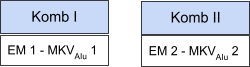
\includegraphics[width=.6\linewidth]{comb_mkv_alu_1}
  \captionof{figure}{Kombinationen von Methoden-Konvertierungsvarianten AIu}
  \label{abb:comb_mkv_alu_1}

\end{minipage}%
\hspace{.04\linewidth}% Abstand zwischen Bilder
\begin{minipage}[b]{.58\linewidth}


  \centering
  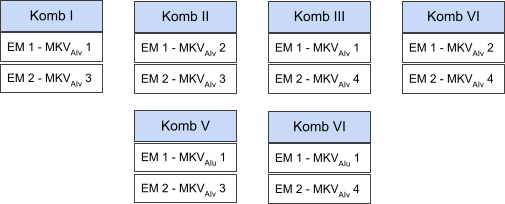
\includegraphics[width=\linewidth]{comb_mkv_alu_alv}
  \captionof{figure}{Kombinationen von Methoden-Konvertierungsvarianten AIu+AIv}
  \label{abb:comb_mkv_alu_alv}

\end{minipage}
\end{figure}


\noindent


\noindent
Im Allgemeinen l�sst sich sagen, dass die Anzahl der Kombinationen von Methoden-Konvertierungsvarianten von der Anzahl der Methoden im erwarteten Interface ($|EM|$) und der Anzahl von Methoden-Konvertierungsvarianten ($|MKV|$), die aus der selektierten Kombination von Typ-Konvertierungsvarianten erzeugt werden k�nnen. Da aus einer Kombination von Methoden-Konvertierungsvarianten jeweils eine ben�tigte Komponente erzeugt werden kann, gilt f�r die Anzahl der ben�tigten Komponenten ($|Komb_{ben}|$) dasselbe. Im schlimmsten Fall berechnet sich die Anzahl der ben�tigten Komponenten wie folgt:
\begin{align*}
|Komb_{ben}| = |Komb_{MKV}| = \frac{|MKV|!}{(|MVK| - |EM|)!*|EM|!}
\end{align*}


\subsubsection{Injizieren der ben�tigten Komponente}\label{sem_eval_step4}
Der Setter f�r die Setter-Injection wird in der Testklasse �ber die Annotation @QueryTypeInstanceSetter ermittelt. Danach wird diese Methode auf dem Testobjekt mit der ben�tigten Komponente als Parameter aufgerufen. 
\subsection{Schritt 5: Durchf�hren der Tests}\label{sem_eval_step5}
Die Testf�lle aus der Testklasse werden �ber die Annotation @QueryTypeTest ermittelt und sequentiell ausgef�hrt. Als Ergebnis der Testausf�hrung f�r eine ben�tigte Komponente wird ein Objekt des Typs TestResult zur�ckgegeben. Tritt bei der Testausf�hrung eine Exception auf, wird diese im TestResult-Objekt hinterlegt. Im Anschluss wird das TestResult-Objekt direkt zur�ckgegeben, um die Ausf�hrung der �brigen Tests zu verhindern. Wenn ein Test mit positivem Ergebnis durchgef�hrt wird, wird das Attribut passedTests im TestResult-Objekt inkrementiert. Sollten alle Tests erfolgreich durchgef�hrt worden sein, wird das TestResult-Objekt zur�ckgegeben.
\myparagraph{Umgang mit kombinierten angebotenen Komponenten}
Ab dem zweiten Durchlauf werden werden die ben�tigten Komponenten in Schritt 3 aus Kombinationen von Typ-Konvertierungsvarianten mehrere angebotener Interfaces erzeugt. Das f�hrt dazu, dass die Methodenaufrufe auf dem erwarteten Interface an unterschiedliche angebotene Komponenten delegiert werden. Hierbei kann der Fall eintreten, dass mehrere dieser Methoden von der Semantik her auf den gleichen Daten operieren m�ssen, die Aufrufe dieser jedoch an unterschiedliche Komponenten delegiert werden, welche auch auf unterschiedlichen Daten operieren.\\\\
Ein Beispiel hierf�r w�re ein Stack, der durch das erwartete Interface Stack beschrieben. Dieses enth�lt eine push und eine pop Methoden mit der ein Element im Stack hinzugef�gt bzw. entfernt werden kann (siehe \abbref{expected_stack}). Hierbei ist anzunehmen, dass die beiden Methoden auf denselben Daten arbeiten, sodass nach dem Hinzuf�gen eines Elements a (push(a)) und dem darauf folgenden Aufruf der Methode pop() als R�ckgabewert wieder das zuvor hinzugef�gte Element a geliefert wird (siehe \abbref{sd_stack_1}). Wenn die beiden Methoden-Aufrufe jedoch an zwei unterschiedliche Objekte StackA und StackB delegiert werden, die auf unterschiedlichen Daten operieren, dann w�rde dieses Verhalten nicht nachgewiesen werden k�nnen (siehe \abbref{sd_stack_2}).

\begin{figure}[H]
\begin{minipage}[b]{.24\linewidth}
  \centering
  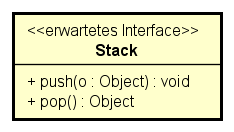
\includegraphics[width=\linewidth]{expected_stack}
  \captionof{figure}{Erwartetes Interface Stack}
  \label{abb:expected_stack}

\end{minipage}%
\hspace{.04\linewidth}% Abstand zwischen Bilder
\begin{minipage}[b]{.72\linewidth}


  \centering
  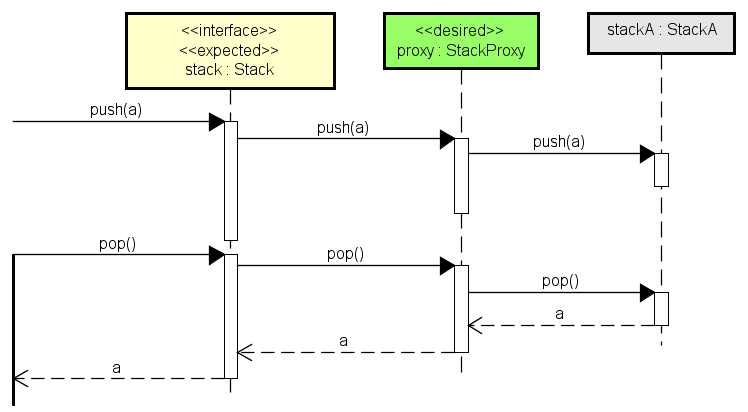
\includegraphics[width=\linewidth]{sd_stack_1}
  \captionof{figure}{Delegation der Stack-Methoden an genau eine angebotene Komponente}
  \label{abb:sd_stack_1}

\end{minipage}
\end{figure}


%\myBigFigure{expected_stack}{Erwartetes Interface Stack}{expected_stack}
%\myBigFigure{sd_stack_1}{Delegation der Stack-Methoden an genau eine angebotene Komponente}{sd_stack_1}
\myBigFigure{sd_stack_2}{Delegation der Stack-Methoden an unterschiedliche angebotene Komponenten}{sd_stack_2}
\noindent
In einem solchen Fall sollte der Zusammenhang dieser erwarteten Methoden in den Tests spezifiziert werden, sodass diese besonderen semantischen Anforderungen in diesem Schritt evaluiert werden k�nnen. \lstref{LST_StackTest} zeigt ein Beispiel bezogen auf das Szenario aus \abbref{sd_stack_1}.
\begin{lstlisting}[{caption = Testklasse f�r ein erwartetes Interfaces Stack
},{label = LST_StackTest}]
public class StackTest {

  private Stack stack;

  @QueryTypeInstanceSetter
  public void setProvider( Stack stack ) {
    this.stack = stack;
  }

  @QueryTypeTest
  public void pushPop() {
    Object a = new Object();
    stack.push( a );
    Object evalObj = stack.pop();
    assertTrue( a == evalObj );
  }

}
\end{lstlisting}

\subsubsection{Schritt 6: Auswertung des Testergebnisses}\label{sem_eval_step6}
Sofern alle Tests erfolgreich durchgelaufen sind, wird die aktuell selektierte ben�tigte Komponente als passend bewertet und als Ergebnis des Explorationsalgorithmus zur�ckgegeben.\\\\
Sollte einer der Tests nicht erfolgreich sein, wird die semantische Evaluation ab Schritt 3 (siehe \ref{sem_eval_step3}) wiederholt. Sofern keine ben�tigten Komponenten mehr erzeugt werden k�nnen, ist die Suche nach einer passenden Komponente gescheitert.\\\\
Da die Suche zur Laufzeit ausgef�hrt wird, reicht es, wenn eine passende Komponente gefunden wird. Selbst wenn es mehrere passende Komponenten geben sollte, g�be es in dem beschriebenen Verfahren keine M�glichkeit festzustellen, welche die semantischen Anforderungen besser erf�llt. Zwar w�ren k�nnte man die passenden Komponenten hinsichtlich der ben�tigten Systemressourcen untersuchen. Aufgrund der Vielzahl von m�glichen Kombinationen (siehe \ref{sem_eval_step2} und \ref{sem_eval_step3}) rechtfertigt der daf�r notwendige Aufwand den daraus resultierenden Performancegewinn vermutlich nicht.
